% !TeX program = lualatex

\documentclass[aspectratio=169]{beamer}

\usepackage{hyperref}
\usepackage{booktabs}
\usepackage{fontspec}
\usepackage{microtype}
\usepackage{palatino}
\usepackage[default]{FiraSans}

\setmonofont{PragmataPro Mono}

\RequirePackage{unicode-math}
\setmathfont{Asana-Math.otf}

\mode<presentation>{
  \usetheme{default}
  \usefonttheme{structurebold}

  \definecolor{structureFG}{HTML}{5C6166}
  \definecolor{structureBG}{HTML}{FCFCFC}
  \definecolor{alert}{HTML}{E65050}
  \definecolor{example}{HTML}{6CBF43}

  \setbeamercolor*{strucure}{fg=structureFG,bg=structureBG}%
  \setbeamercolor*{local strucure}{fg=structureFG,bg=structureBG}%
  \setbeamercolor*{titlelike}{fg=structureFG}%
  \setbeamercolor*{alerted text}{fg=alert}%
  \setbeamercolor*{example text}{fg=example}%

  \setbeamercolor*{caption name}{fg=structureFG}%
  \setbeamercolor*{block title}{fg=structureFG}%
  \setbeamercolor*{itemize item}{fg=structureFG}%
  \setbeamercolor*{itemize subitem}{fg=structureFG}%
  \setbeamercolor*{itemize subsubitem}{fg=structureFG}%
  \setbeamercolor*{enumerate item}{fg=structureFG}%
  \setbeamercolor*{enumerate subitem}{fg=structureFG}%
  \setbeamercolor*{enumerate subsubitem}{fg=structureFG}%

  \setbeamercolor*{navigation symbols}{fg=structureFG!50}
  \setbeamercolor*{navigation symbols dimmed}{fg=structureFG!15}

  \setbeamertemplate{footline}[frame number]
  \setbeamertemplate{headline}{}
}

\usepackage{twemojis}
\usepackage{fancyvrb}
\usepackage{listings}
\lstset{
  inputencoding=utf8,
  basicstyle=\linespread{1.0}\ttfamily\mdseries,
  fancyvrb=true,
  sensitive=true,
  %breaklines=true,
  extendedchars=false,
  showstringspaces=false,
  columns=fixed,
  stepnumber=1,
  escapeinside={\%*}{*)},
  lineskip=-5pt,
  basewidth=0.5em
}

\definecolor {codeBackground} {HTML} {F4F4F4} % {F7F7F7} AYU common.bg
\definecolor {codeForeground} {HTML} {000000} % AYU common.fg
\definecolor {codeKeyword}    {HTML} {399EE6} % AYU syntax.entity
\definecolor {codeBuiltin}    {HTML} {55B4D4} % AYU syntax.tag
\definecolor {codeConstant}   {HTML} {A37ACC} % AYU syntax.constant
\definecolor {codeString}     {HTML} {86B300} % AYU syntax.string
\definecolor {codeEmph}       {HTML} {FA8D3E} % AYU syntax.keyword
\definecolor {codeRuler}      {HTML} {CACACA} % AYU ui.panel.border
\definecolor {codeComment}    {HTML} {8A9199} % AYU common.ui
\definecolor {codeIdentifier} {HTML} {1c1c1c}
\definecolor {codeOperator}   {HTML} {4CBF99}
\definecolor {codeError}      {HTML} {E65050} % AYU common.error

\definecolor{pc}{HTML}{55B4D4}
\definecolor{branching}{HTML}{FA8D3E}
\definecolor{arithmetic}{HTML}{ED9366}
\definecolor{stack}{HTML}{A37ACC}
\definecolor{userio}{HTML}{4CBF99}
\definecolor{gridio}{HTML}{86B300}
\definecolor{stringmode}{HTML}{FF7383}
\definecolor{endprogram}{HTML}{E65050}
\definecolor{ignore}{HTML}{787B80}
\definecolor{number}{HTML}{5C6166}
\definecolor{codebg}{HTML}{F3F4F5}

\colorlet{stringbg}{stringmode!20}
\colorlet{pcbg}{pc!20}
\colorlet{branchingbg}{branching!20}

\lstdefinelanguage{sql}{
  basicstyle=\linespread{1.0}\color{codeForeground}\ttfamily\mdseries,
  identifierstyle=\color{codeIdentifier},
  commentstyle=\color{codeComment},
  stringstyle=\color{codeString},
  emphstyle={\color{codeEmph}\itshape\bfseries},
  keywordstyle={[1]\color{codeKeyword}\bfseries},
  keywordstyle={[2]\color{codeBuiltin}\bfseries},
  keywordstyle={[3]\color{codeConstant}\bfseries},
  keywordstyle={[4]\color{codeOperator}\bfseries},
  emptylines=*10,
  morestring=[d]{'},
  morecomment=[l]{--},
  morekeywords=[1]{WITH,RECURSIVE,UNION,ALL,SELECT,FROM,WHERE,LATERAL,AS,ITERATE,LEFT,RIGHT,OUTER,INNER,JOIN},
  morekeywords=[2]{int4,float8,text,boolean,ARRAY,CARDINALITY,ABS,FLOOR,CEIL,ROUND,RANDOM,SIGN,MAX,MIN,ARRAY_AGG,unnest,json_each},
  morekeywords=[3]{NULL,TRUE,FALSE},
  morekeywords=[4]{AND,OR,NOT,BETWEEN,CASE,WHEN,THEN,END,IS},
  literate=%
    {(}{{{\color{codeOperator}(}}}1
    {)}{{{\color{codeOperator})}}}1
    {[}{{{\color{codeOperator}[}}}1
    {]}{{{\color{codeOperator}]}}}1
    % {\{}{{{\color{codeOperator}\{}}1
    % {\}}{{{\color{codeOperator}\}}}1
    {:}{{{\color{codeOperator}:}}}1
    {.}{{{\color{codeOperator}.}}}1
    {,}{{{\color{codeOperator},}}}1
    {+}{{{\color{codeOperator}+}}}1
    {-}{{{\color{codeOperator}-}}}1
    {*}{{{\color{codeOperator}*}}}1
    {/}{{{\color{codeOperator}/}}}1
    {\%}{{{\color{codeOperator}\%{}}}}1
    {@}{{{\color{codeOperator}@}}}1
    {^}{{{\color{codeOperator}\^{}}}}1
    {|}{{{\color{codeOperator}|}}}1
    {\&}{{{\color{codeOperator}\&}}}1
    {<}{{{\color{codeOperator}<}}}1
    {>}{{{\color{codeOperator}>}}}1
    {=}{{{\color{codeOperator}=}}}1
    {!}{{{\color{codeOperator}!}}}1
    {...}{{{\color{codeComment}...}}}3
}
\newcommand{\sql}[1]{\text{\lstinline[language=sql]!#1!}}

\lstdefinelanguage{py}{
  basicstyle=\linespread{1.0}\color{codeForeground}\ttfamily,
  identifierstyle=\color{codeIdentifier},
  commentstyle=\color{codeComment},
  stringstyle=\color{codeString},
  emphstyle={\color{codeEmph}\itshape\bfseries},
  keywordstyle={[1]\color{codeKeyword}\bfseries},
  keywordstyle={[2]\color{codeBuiltin}\bfseries},
  keywordstyle={[3]\color{codeConstant}\bfseries},
  keywordstyle={[4]\color{codeOperator}\bfseries},
  emptylines=*10,
  morestring=[d]{"},
  morecomment=[l]{\#},
  morekeywords=[1]{def,for,while,if,else,try,except,finally,yield,async,await,return,match,case},
  morekeywords=[2]{int,float,bool,str,list,dict,set},
  morekeywords=[3]{None,True,False},
  morekeywords=[4]{is,not,in,and,or},
  literate=%
    {(}{{{\color{codeOperator}(}}}1
    {)}{{{\color{codeOperator})}}}1
    {[}{{{\color{codeOperator}[}}}1
    {]}{{{\color{codeOperator}]}}}1
    % {\{}{{{\color{codeOperator}\{}}1
    % {\}}{{{\color{codeOperator}\}}}1
    {:}{{{\color{codeOperator}:}}}1
    {.}{{{\color{codeOperator}.}}}1
    {,}{{{\color{codeOperator},}}}1
    {+}{{{\color{codeOperator}+}}}1
    {-}{{{\color{codeOperator}-}}}1
    {*}{{{\color{codeOperator}*}}}1
    {/}{{{\color{codeOperator}/}}}1
    {\%}{{{\color{codeOperator}\%{}}}}1
    {@}{{{\color{codeOperator}@}}}1
    {^}{{{\color{codeOperator}\^{}}}}1
    {|}{{{\color{codeOperator}|}}}1
    {\&}{{{\color{codeOperator}\&}}}1
    {<}{{{\color{codeOperator}<}}}1
    {>}{{{\color{codeOperator}>}}}1
    {==}{{{\color{codeOperator}==}}}2
    {!=}{{{\color{codeOperator}!=}}}2
    {<=}{{{\color{codeOperator}<=}}}2
    {>=}{{{\color{codeOperator}>=}}}2
    {...}{{{\color{codeComment}...}}}3
    {=}{{{\color{codeConstant}=}}}1
}
\newcommand{\py}[1]{\text{\lstinline[language=py]!#1!}}

\lstdefinelanguage{befunge}{
  basicstyle=\ttfamily\mdseries\color{ignore},
  literate=%
    {^}{{{\color{pc}\^{}}}}1
    {<}{{{\color{pc}<}}}1
    {>}{{{\color{pc}>}}}1
    {v}{{{\color{pc}v}}}1
    {?}{{{\color{pc}?}}}1
    {\#}{{{\color{pc}\#}}}1
    {|}{{{\color{branching}|}}}1
    {\_}{{{\color{branching}\_}}}1
    {+}{{{\color{arithmetic}+}}}1
    {-}{{{\color{arithmetic}-}}}1
    {*}{{{\color{arithmetic}*}}}1
    {/}{{{\color{arithmetic}/}}}1
    {\%}{{{\color{arithmetic}\%{}}}}1
    {\!}{{{\color{arithmetic}!}}}1
    {\`}{{{\color{arithmetic}\`{}}}}1
    {:}{{{\color{stack}:}}}1
    {\\}{{{\color{stack}\textbackslash}}}1
    {\$}{{{\color{stack}\$}}}1
    {.}{{{\color{userio}.}}}1
    {,}{{{\color{userio},}}}1
    {&}{{{\color{userio}\&}}}1
    {~}{{{\color{userio}\~{}}}}1
    {g}{{{\color{gridio}g}}}1
    {p}{{{\color{gridio}p}}}1
    {"}{{{\color{stringmode}"}}}1
    {@}{{{\color{endprogram}@}}}1
    {0}{{{\color{number}0}}}1
    {1}{{{\color{number}1}}}1
    {2}{{{\color{number}2}}}1
    {3}{{{\color{number}3}}}1
    {4}{{{\color{number}4}}}1
    {5}{{{\color{number}5}}}1
    {6}{{{\color{number}6}}}1
    {7}{{{\color{number}7}}}1
    {8}{{{\color{number}8}}}1
    {9}{{{\color{number}9}}}1
}
\newcommand{\befunge}[1]{\text{\lstinline[basicstyle=\ttfamily\mdseries\small,language=befunge]!#1!}}
\lstMakeShortInline[columns=fixed,language=befunge]§
\newcommand{\stringStyle}[1]{{\lstinline[basicstyle=\ttfamily\mdseries\color{stringmode}]!#1!}}

\lstdefinelanguage{brainfuck}{
  basicstyle=\ttfamily\mdseries\color{ignore},
  literate=%
    {<}{{{\color{pc}<}}}1
    {>}{{{\color{pc}>}}}1
    {[}{{{\color{branching}[}}}1
    {]}{{{\color{branching}]}}}1
    {+}{{{\color{arithmetic}-}}}1
    {-}{{{\color{arithmetic}-}}}1
    {.}{{{\color{userio}.}}}1
    {,}{{{\color{userio},}}}1
}

\usepackage{adjustbox}

%% TikZ ist kein Zeichenprogramm
\usepackage{tikz}
\usetikzlibrary{arrows.meta}
\usetikzlibrary{patterns}
\usetikzlibrary{shapes.symbols}
\usetikzlibrary{shapes.multipart}
\usetikzlibrary{shapes.misc}
\usetikzlibrary{shadows}
\usetikzlibrary{shadings}
\usetikzlibrary{calc}
\usetikzlibrary{decorations.pathreplacing}
%% layered TiKZ drawings
\pgfdeclarelayer{background}
\pgfdeclarelayer{foreground}
\pgfsetlayers{background,main,foreground}
%% TikZ-based (scatter) plots
\usepackage{pgfplots}
%% read table cells from CSV input
\usepackage{pgfplotstable}
\usepackage{pgffor}
\usetikzlibrary{fpu}
%% make sure that TikZ's calc library and lstlisting's 'mathescape=true' cooperate
\makeatletter
\global\let\tikz@ensure@dollar@catcode=\relax
\makeatother

%% lengths that measure character box width and height in code/in a listing
\newlength{\x}
\newlength{\y}
\newlength{\xx}


\title[Befunge]{Befunge-93 in SQL}
\subtitle{(Ab-)Using SQLs Turing Completeness}
\author[Tim F.]{Tim Fischer}
\institute[TUE]{Eberhard Karls Universität Tübingen \\ \smallskip \textit{t.fischer@student.uni-tuebingen.de}}
\date[\today]{SQL is a Programming Language \\ \today}

\begin{document}

\begin{frame}
  \titlepage
\end{frame}

\begin{frame}
  \frametitle{Befunge TL;DR}

  \begin{columns}[c]
    \begin{column}{0.45\textwidth}
      Befunge is a...
      \begin{itemize}
        \item stack-based
        \item Turing complete
        \item two-dimensional
        \item self-modifying
        \item imperative
        \item esoteric
        \item programming language.
      \end{itemize}
    \end{column}
  \end{columns}
\end{frame}

\begin{frame}[fragile]
  \frametitle{Befunge Commands}
  \small

  \begin{table}
    \begin{adjustbox}{center}
      \begin{tabular}{cl}
        \textbf{Commands}                     & \textbf{Description}                           \\
        \midrule
        \befunge{>v<^}                        & Set direction of program counter               \\
        \befunge{#}                           & Skip the next command                          \\
        \befunge{?}                           & Set direction of program counter at random     \\
        \befunge{_|}                          & Vertical and horizontal branching              \\
        \befunge{0123456789}                  & Put number on stack                            \\
        \befunge{:\$\\} & Stack modification                             \\
        \befunge{+-*/\%\!}                    & Arithmetic operators                           \\
        \befunge{.,}                          & Output either numeric or ASCII value to stdout \\
        \befunge{\&~}                         & Take either numeric or ASCII value from stdin  \\
        \befunge{gp}                          & Get or put ASCII value from the grid           \\
        \befunge{"}                           & Toggle string mode                             \\
        \befunge{@}                           & Halt program execution                         \\
      \end{tabular}
    \end{adjustbox}
  \end{table}
\end{frame}

\begin{frame}[fragile]
  \frametitle{Simple Examples}

  \begin{columns}[c]
    \begin{column}{0.45\textwidth}
      \begin{figure}[t]
        \begin{adjustbox}{center}
          \centering
          \small
          %% measure the width of xx in a listing
          \settowidth{\xx}{\lstinline[columns=fixed]{xx}}\setlength{\x}{0.5\xx}
          \setlength{\y}{2ex}
          \begin{tikzpicture}[x=\x,y=-\y,inner sep=0mm]
            \node[anchor=north west] at (0,0) {%
              \begin{lstlisting}[language=befunge,gobble=16]
                "!dlroW ,olleH">:#v_@
                               ^ ,<
              \end{lstlisting}%
            };
            \begin{pgfonlayer}{background}
              \fill[codebg,rounded corners=1pt] (-1,-0.5) rectangle (22,2.5);
            \end{pgfonlayer}
          \end{tikzpicture}
        \end{adjustbox}
        \caption{Hello World}
      \end{figure}
    \end{column}

    \begin{column}{0.45\textwidth}
      \begin{figure}[t]
        \begin{adjustbox}{center}
          \centering
          \small
          %% measure the width of xx in a listing
          \settowidth{\xx}{\lstinline[columns=fixed]{xx}}\setlength{\x}{0.5\xx}
          \setlength{\y}{2ex}
          \begin{tikzpicture}[x=\x,y=-\y,inner sep=0mm]
            \node[anchor=north west] at (0,0) {%
              \begin{lstlisting}[language=befunge,gobble=16]
                &>:1-:v v *_$.@
                 ^    _$>\:^
              \end{lstlisting}%
            };
            \begin{pgfonlayer}{background}
              \fill[codebg,rounded corners=1pt] (-1,-0.5) rectangle (16,2.7);
            \end{pgfonlayer}
          \end{tikzpicture}
        \end{adjustbox}
        \caption{Factorial}
      \end{figure}
    \end{column}
  \end{columns}
\end{frame}

\begin{frame}[fragile]
  \frametitle{Examples}

  \begin{figure}[t]
    \begin{adjustbox}{center}
      \centering
      \footnotesize
      %% measure the width of xx in a listing
      \settowidth{\xx}{\lstinline[columns=fixed]{xx}}\setlength{\x}{0.5\xx}
      \setlength{\y}{2ex}
      \begin{tikzpicture}[x=\x,y=-\y,inner sep=0mm]
        \node[anchor=north west] at (0,0) {%
          \begin{lstlisting}[language=befunge,gobble=12]
            211p&01p>121p          >21g1+21p 11g21g-v>11g21g%#v_v
                                                    >|
                             v,,,,, ,,,.g11"is prime"<
            >       ^        >   v ^                          <
            ^_@#-g10p11:+1g11,*25<,,,,,,,,,,,,.g11"is not prime"<
        \end{lstlisting}%
        };
        \begin{pgfonlayer}{background}
          \fill[codebg,rounded corners=1pt] (-1,-0.5) rectangle (54,6);
        \end{pgfonlayer}
      \end{tikzpicture}
    \end{adjustbox}
    \caption{Calculating Prime Numbers}
  \end{figure}
\end{frame}

\begin{frame}[fragile]
  \frametitle{Interpreter Pseudocode}

  \begin{figure}[t]
    \centering
    \small
    %% measure the width of xx in a listing
    \settowidth{\xx}{\lstinline[columns=fixed]{xx}}\setlength{\x}{0.5\xx}
    \setlength{\y}{2ex}
    \begin{tikzpicture}[x=\x,y=-\y,inner sep=0mm]
      \node[anchor=north west] at (0,0) {%
        \begin{lstlisting}[language=py,gobble=10]
          def interpreter(source):
            program = preprocess(source)
            state   = make_inital_state(program)

            while not state.done():
              match state.mode:
                case "%*\twemoji{gear}*)": ...
                case "%*\twemoji{sewing needle}*)": ...

              match state.direction:
                case "%*\twemoji{right arrow}*)": ...
                case "%*\twemoji{down arrow}*)": ...
                case "%*\twemoji{left arrow}*)": ...
                case "%*\twemoji{up arrow}*)": ...

            return state.result
        \end{lstlisting}%
      };
      \begin{pgfonlayer}{background}
        \fill[codebg,rounded corners=2pt] (-1.0,-0.5) rectangle (39,16);
      \end{pgfonlayer}
    \end{tikzpicture}
  \end{figure}
\end{frame}

\begin{frame}[fragile]
  \frametitle{Types of Control Flow}

  \begin{figure}[t]
    \centering
    \small
    %% measure the width of xx in a listing
    \settowidth{\xx}{\lstinline[columns=fixed]{xx}}\setlength{\x}{0.5\xx}
    \setlength{\y}{2ex}
    \begin{tikzpicture}[x=\x,y=-\y,inner sep=0mm]
      \node[anchor=north west] at (0,0) {%
        \begin{lstlisting}[language=py,gobble=10]
          def interpreter(source):
            program = preprocess(source)
            state   = make_inital_state(program)

            while not state.done():
              match state.mode:
                case "%*\twemoji{gear}*)": ...
                case "%*\twemoji{sewing needle}*)": ...

              match state.direction:
                case "%*\twemoji{right arrow}*)": ...
                case "%*\twemoji{down arrow}*)": ...
                case "%*\twemoji{left arrow}*)": ...
                case "%*\twemoji{up arrow}*)": ...

            return state.result
        \end{lstlisting}%
      };
      \begin{pgfonlayer}{background}
        \begin{scope}[rounded corners=2pt]
          \fill[codebg]                                          (-1.00,-0.50) rectangle (40.00,16.00);
          \fill[codeEmph,draw=codeEmph,line width=1.7pt]         ( 0.25, 1.15) rectangle (38.75, 3.30);
          \fill[codeEmph!25]                                     ( 1.50, 1.15) rectangle (38.75, 3.30);
          \fill[codeConstant,draw=codeConstant,line width=1.7pt] ( 0.25, 3.90) rectangle (38.75,14.00);
          \fill[codeConstant!25]                                 ( 1.50, 3.90) rectangle (38.75,14.00);
          \fill[codeString,draw=codeString,line width=1.7pt]     ( 2.25, 5.00) rectangle (37.75, 8.00);
          \fill[codeString!25]                                   ( 3.55, 5.00) rectangle (37.75, 8.00);
          \fill[codeString,draw=codeString,line width=1.7pt]     ( 2.25, 8.70) rectangle (37.75,13.75);
          \fill[codeString!25]                                   ( 3.55, 8.70) rectangle (37.75,13.75);
        \end{scope}
        \begin{scope}[inner sep=1pt]
          \node[codeEmph!25]     at (0.85,1.65) {\texttt{↓}};
          \node[codeConstant!25] at (0.85,4.50) {\texttt{↺}};
          \node[codeString!25]   at (2.85,5.50) {\texttt{⥥}};
          \node[codeString!25]   at (2.85,9.20) {\texttt{⥥}};
        \end{scope}
      \end{pgfonlayer}
    \end{tikzpicture}
  \end{figure}
\end{frame}

\begin{frame}[fragile]
  \frametitle{{\color{codeEmph} Non-Branching Linear Control Flow} in SQL}

  \begin{columns}[c]
    \begin{column}{0.65\textwidth}
      \begin{figure}[t]
        \centering
        \small
        %% measure the width of xx in a listing
        \settowidth{\xx}{\lstinline[columns=fixed]{xx}}\setlength{\x}{0.5\xx}
        \setlength{\y}{2ex}
        \begin{tikzpicture}[x=\x,y=-\y,inner sep=0mm]
          \node[anchor=north west] at (0,0) {%
            \begin{lstlisting}[language=sql,gobble=14]
              SELECT ...
              FROM   LATERAL (
                        preprocess(source)
                     ) AS _1(program),
                     LATERAL (
                        make_inital_state(program)
                     ) AS _2(state)
            \end{lstlisting}%
          };
          \begin{pgfonlayer}{background}
            \begin{scope}[rounded corners=2pt]
              \fill[codebg]                                          (-1.00,-0.50) rectangle (39.00,8.00);

              \fill[codeEmph,draw=codeEmph,line width=1.7pt]         ( 5.25, 1.10) rectangle (37.25,7.50);
              \fill[codeEmph!25]                                     ( 6.50, 1.10) rectangle (37.25,7.50);

              \fill[codeOperator,draw=codeOperator,line width=1.7pt] ( 8.50, 2.10) rectangle (36.25,3.20);
              \fill[codeOperator!25]                                 ( 9.75, 2.10) rectangle (36.25,3.20);
              \fill[codeOperator,draw=codeOperator,line width=1.7pt] ( 8.50, 5.30) rectangle (36.25,6.40);
              \fill[codeOperator!25]                                 ( 9.75, 5.30) rectangle (36.25,6.40);
            \end{scope}
            \node[inner sep=1pt,codeEmph!25] at (5.825,1.70) {\texttt{↓}};
            \begin{scope}[inner sep=1pt,every node/.style={codeOperator!25}]
              \node at (9.075,2.75) {\texttt{↦}};
              \node at (9.075,5.95) {\texttt{↦}};
            \end{scope}
          \end{pgfonlayer}
        \end{tikzpicture}
      \end{figure}
    \end{column}
    \begin{column}{0.35\textwidth}
      \begin{figure}
        \centering
        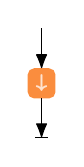
\begin{tikzpicture}[x=10mm,y=-7mm,inner sep=1pt]
          %% query parts
          \node[codeEmph!25,draw=codeEmph,fill=codeEmph,rounded corners=2pt,inner sep=2pt,line width=0.8pt] at (0,0.0) (start) {\texttt{↓}};
          %% transitions (through check)
          \begin{scope}[goto/.tip={Latex[round,length=2mm]},return/.tip={Latex[round,length=2mm] Bar}]
            \draw[{goto}-]   (start) to +(0,-1.0);
            \draw[-{return}] (start) to +(0, 1.0);
          \end{scope}
        \end{tikzpicture}
      \end{figure}
    \end{column}
  \end{columns}
\end{frame}

\begin{frame}[fragile]
  \frametitle{{\color{codeConstant} Condition-controlled Non-Linear Control Flow} in SQL}

  \begin{columns}[c]
    \begin{column}{0.65\textwidth}
      \begin{figure}[t]
        \centering
        \small
        %% measure the width of xx in a listing
        \settowidth{\xx}{\lstinline[columns=fixed]{xx}}\setlength{\x}{0.5\xx}
        \setlength{\y}{2ex}
        \begin{tikzpicture}[x=\x,y=-\y,inner sep=0mm]
          \node[anchor=north west] at (0,0) {%
            \begin{lstlisting}[language=sql,gobble=14]
              WITH RECURSIVE
                loop(...) AS (

                  SELECT  %*\,{\color{codeComment}\itshape init}*)

                    UNION

                  SELECT  %*\,{\color{codeComment}\itshape body}*)
                  FROM    loop AS state
                  WHERE   NOT state.done()

                )
              SELECT ...
              FROM   loop
              WHERE  ...
            \end{lstlisting}%
          };
          \begin{pgfonlayer}{background}
            \begin{scope}[rounded corners=2pt]
              \fill[codebg]                                          (-1.00,-0.5) rectangle (30,14.3);

              \fill[codeEmph,draw=codeEmph,line width=1.7pt]         ( 2.50, 2.5) rectangle (29, 3.9);
              \fill[codeEmph!25]                                     ( 3.75, 2.5) rectangle (29, 3.9);

              \fill[codeOperator,draw=codeOperator,line width=1.7pt] (10.50, 2.7) rectangle (28, 3.7);
              \fill[codeOperator!25]                                 (11.75, 2.7) rectangle (28, 3.7);

              \fill[codeConstant,draw=codeConstant,line width=1.7pt] ( 2.50, 5.9) rectangle (29, 9.4);
              \fill[codeConstant!25]                                 ( 3.75, 5.9) rectangle (29, 9.4);

              \fill[codeOperator,draw=codeOperator,line width=1.7pt] (10.50, 6.1) rectangle (28, 7.1);
              \fill[codeOperator!25]                                 (11.75, 6.1) rectangle (28, 7.1);

              \fill[codeOperator,draw=codeOperator,line width=1.7pt] (10.50, 8.2) rectangle (28, 9.2);
              \fill[codeOperator!25]                                 (11.75, 8.2) rectangle (28, 9.2);
            \end{scope}
            \begin{scope}[inner sep=1pt]
              \node[codeEmph!25]     at ( 3.125,3.2) {\texttt{↓}};
              \node[codeOperator!25] at (11.125,3.3) {\texttt{↦}};
              \node[codeConstant!25] at ( 3.125,6.6) {\texttt{↺}};
              \node[codeOperator!25] at (11.125,6.6) {\texttt{↦}};
              \node[codeOperator!25] at (11.125,8.7) {\texttt{↦}};
            \end{scope}
          \end{pgfonlayer}
        \end{tikzpicture}
      \end{figure}
    \end{column}
    \begin{column}{0.35\textwidth}
      \begin{figure}
        \centering
        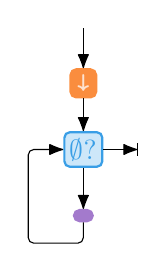
\begin{tikzpicture}[x=10mm,y=-7mm,inner sep=1pt]
          %% query parts
          \begin{scope}[every node/.style={rounded corners=2pt,inner sep=2pt,line width=0.8pt}]
            \node[codeEmph!25,draw=codeEmph,fill=codeEmph]             at (0,0.0) (start) {\texttt{↓}};
            \node[codeKeyword,draw=codeKeyword,fill=codeKeyword!25]    at (0,1.2) (check) {$\emptyset$?};
            \node[codeConstant!25,draw=codeConstant,fill=codeConstant] at (0,2.4) (step)  {\texttt{↺}};
          \end{scope}
          \coordinate (through) at (-0.7,2.9);
          %% transitions (through check)
          \begin{scope}[goto/.tip={Latex[round,length=2mm]},return/.tip={Latex[round,length=2mm] Bar}]
            \draw[{goto}-]   (start) to +(0,-1.0);
            \draw[-{goto}]   (start) to (check);
            \draw[-{return}] (check) to +(0.7,0);
            \draw[-{goto}]   (check) to (step);
            %% back-to-check transitions
            \begin{scope}[rounded corners=2pt]
              \draw[-{goto}] (step) to (step |- through) to (through) to (through |- check) to (check);
            \end{scope}
          \end{scope}
        \end{tikzpicture}
      \end{figure}
    \end{column}
  \end{columns}
\end{frame}

\begin{frame}[fragile]
  \frametitle{{\color{codeString} Branching Linear Control Flow} in SQL}

  \begin{columns}[c]
    \begin{column}{0.65\textwidth}
      \begin{figure}[t]
        \centering
        \scriptsize
        %% measure the width of xx in a listing
        \settowidth{\xx}{\lstinline[columns=fixed]{xx}}\setlength{\x}{0.5\xx}
        \setlength{\y}{2ex}
        \begin{tikzpicture}[x=\x,y=-\y,inner sep=0mm]
          \node[anchor=north west] at (0,0) {%
            \begin{lstlisting}[language=sql,gobble=14]
              SELECT ...
              FROM   loop AS state,

              LATERAL (
                SELECT  ... WHERE mode='%*\twemoji{gear}*)'
                  UNION ALL
                SELECT  ... WHERE mode='%*\twemoji{sewing needle}*)'
              ) AS next,

              LATERAL (
                SELECT  ... WHERE direction='%*\twemoji{right arrow}*)'
                  UNION ALL
                SELECT  ... WHERE direction='%*\twemoji{down arrow}*)'
                  UNION ALL
                SELECT  ... WHERE direction='%*\twemoji{left arrow}*)'
                  UNION ALL
                SELECT  ... WHERE direction='%*\twemoji{up arrow}*)'
              ) AS move
            \end{lstlisting}%
          };
          \begin{pgfonlayer}{background}
            \begin{scope}[rounded corners=2pt]
              \fill[codebg]                                          (-5.5, -1.00) rectangle (36.5, 20.00);

              \fill[codeConstant,draw=codeConstant,line width=1.7pt] (-4.0, -0.00) rectangle (35.0, 19.20);
              \fill[codeConstant!25]                                 (-2.5, -0.00) rectangle (35.0, 19.20);

              \fill[codeString,draw=codeString,line width=1.7pt]     (-2.0,  2.60) rectangle (34.0,  8.20);
              \fill[codeString!25]                                   (-0.5,  2.60) rectangle (34.0,  8.20);

              \fill[codeString,draw=codeString,line width=1.7pt]     (-2.0,  8.70) rectangle (34.0, 18.60);
              \fill[codeString!25]                                   (-0.5,  8.70) rectangle (34.0, 18.60);

              \fill[codeOperator,draw=codeOperator,line width=1.7pt] ( 8.5,  3.85) rectangle (13.0,  4.85);
              \fill[codeOperator!25]                                 (10.0,  3.85) rectangle (13.0,  4.85);

              \fill[codeOperator,draw=codeOperator,line width=1.7pt] ( 8.5,  6.10) rectangle (13.0,  7.10);
              \fill[codeOperator!25]                                 (10.0,  6.10) rectangle (13.0,  7.10);

              \fill[codeOperator,draw=codeOperator,line width=1.7pt] ( 8.5, 10.00) rectangle (13.0, 11.00);
              \fill[codeOperator!25]                                 (10.0, 10.00) rectangle (13.0, 11.00);

              \fill[codeOperator,draw=codeOperator,line width=1.7pt] ( 8.5, 12.15) rectangle (13.0, 13.15);
              \fill[codeOperator!25]                                 (10.0, 12.15) rectangle (13.0, 13.15);

              \fill[codeOperator,draw=codeOperator,line width=1.7pt] ( 8.5, 14.30) rectangle (13.0, 15.30);
              \fill[codeOperator!25]                                 (10.0, 14.30) rectangle (13.0, 15.30);

              \fill[codeOperator,draw=codeOperator,line width=1.7pt] ( 8.5, 16.45) rectangle (13.0, 17.45);
              \fill[codeOperator!25]                                 (10.0, 16.45) rectangle (13.0, 17.45);
            \end{scope}
            \begin{scope}[inner sep=1pt]
              \node[codeConstant!25] at (-3.25, 0.5) {\footnotesize \texttt{↺}};
              \node[codeString!25]   at (-1.25, 3.2) {\footnotesize \texttt{⥥}};
              \node[codeString!25]   at (-1.25, 9.3) {\footnotesize \texttt{⥥}};

              \node[codeOperator!25] at ( 9.25, 4.40) {\texttt{↦}};
              \node[codeOperator!25] at ( 9.25, 6.65) {\texttt{↦}};
              \node[codeOperator!25] at ( 9.25,10.55) {\texttt{↦}};
              \node[codeOperator!25] at ( 9.25,12.65) {\texttt{↦}};
              \node[codeOperator!25] at ( 9.25,14.85) {\texttt{↦}};
              \node[codeOperator!25] at ( 9.25,17.00) {\texttt{↦}};
            \end{scope}
          \end{pgfonlayer}
        \end{tikzpicture}
      \end{figure}
    \end{column}
    \begin{column}{0.35\textwidth}
      \begin{figure}
        \centering
        \settowidth{\xx}{\twemoji{rocket}\twemoji{rocket}}\setlength{\x}{0.5\xx}
        \setlength{\y}{2ex}
        
\begin{tikzpicture}[x=\x,y=-\y,inner sep=1pt]
          %% query parts
          \begin{scope}[every node/.style={rounded corners=2pt,inner sep=2pt}]
            \node[codeEmph,fill=codeEmph!25] at ( 0.0,0.0) (start) {\twemoji{gear}\,\twemoji{right arrow}};
            \node[codeKeyword,draw=codeKeyword,fill=codeKeyword!25,line width=0.9pt] at (0,2.0) (check) {$\emptyset$?};
          \end{scope}
          \begin{scope}[every node/.style={codeString,fill=codeString!25,rounded corners=2pt,inner sep=2pt}]
            \node at (-0.835,4.0) (process) {\twemoji{gear}};
            \node at ( 0.835,4.0) (string)  {\twemoji{sewing needle}};

            \node at (-2.505,6.0) (right)   {\twemoji{right arrow}};
            \node at (-0.835,6.0) (down)    {\twemoji{down arrow}};
            \node at ( 0.835,6.0) (left)    {\twemoji{left arrow}};
            \node at ( 2.505,6.0) (up)      {\twemoji{up arrow}};
          \end{scope}
          \coordinate (through1) at (0,2.75);
          \coordinate (through2) at (0,4.75);
          \coordinate (through3) at (-4.5,7.25);

          %% transitions (through check)
          \begin{scope}[rounded corners=2pt,goto/.tip={Latex[round,length=2mm]},return/.tip={Latex[round,length=2mm] Bar}]
            \draw[{goto}-]   (start)   to +(0,-1.5);
            \draw[-{goto}]   (start)   to (check);
            \draw[-{return}] (check)   to +(2.5,0);

            \draw[-{goto}]   (check)   to (through1) to (process |- through1) to (process);
            \draw[-{goto}]   (check)   to (through1) to (string |- through1)  to (string);

            \draw[-{goto}]   (process)                                                 to (down);
            \draw[-{goto}]   (process) to (process |- through2) to (up |- through2)    to (up);

            \draw[-{goto}]   (string)  to (string |- through2)  to (right |- through2) to (right);
            \draw[-{goto}]   (string)                                                  to (left);

            \draw[-{goto}]       (up)    to (up    |- through3) to (through3) to (through3 |- check) to (check);
            \draw[shorten >=2pt] (left)  to (left  |- through3) to (through3);
            \draw[shorten >=2pt] (down)  to (down  |- through3) to (through3);
            \draw[shorten >=2pt] (right) to (right |- through3) to (through3);
          \end{scope}

          \fill[black,radius=1.25pt] ( 0.000, 2.75) circle node (branch1) {};
          \fill[black,radius=1.25pt] (-0.835, 4.75) circle node (branch2) {};
          \fill[black,radius=1.25pt] ( 0.835, 4.75) circle node (branch3) {};

          \begin{pgfonlayer}{background}
            \begin{scope}[rounded corners=2pt]
              \fill[codeEmph,draw=codeEmph,line width=1.7pt]         (-1.4,-0.50) rectangle (2.5,0.50);

              \fill[codeConstant,draw=codeConstant,line width=1.7pt] (-3.7, 3.25) rectangle (5.9,6.75);
              \fill[codeConstant!25]                                 (-3.7, 3.25) rectangle (4.8,6.75);

              \fill[codeString,draw=codeString,line width=1.7pt]     (-1.6, 3.50) rectangle (2.7,4.50);
              \fill[codeString,draw=codeString,line width=1.7pt]     (-3.3, 5.50) rectangle (4.4,6.50);
            \end{scope}
            \node[codeEmph!25]     at (1.9, 0.00) {\texttt{↓}};
            \node[codeConstant!25] at (5.4, 3.75) {\texttt{↺}};
            \node[codeString!25]   at (2.2, 4.00) {\texttt{⥥}};
            \node[codeString!25]   at (3.9, 6.00) {\texttt{⥥}};
          \end{pgfonlayer}
        \end{tikzpicture}
      \end{figure}
    \end{column}
  \end{columns}
\end{frame}

\end{document}

\begin{frame}[fragile]
  \frametitle{Step Function Shape}

  \begin{figure}[t]
    \centering
    \small
    %% measure the width of xx in a listing
    \settowidth{\xx}{\lstinline[columns=fixed]{xx}}\setlength{\x}{0.5\xx}
    \setlength{\y}{2ex}
    \begin{tikzpicture}[x=\x,y=-\y,inner sep=0mm]
      \node[anchor=north west] at (0,0) {%
        \begin{lstlisting}[language=py,gobble=10]
          def step(state):
            match state.mode:
              case "%*\twemoji{gear}*)": ...
              case "%*\twemoji{sewing needle}*)": ...

            match state.direction:
              case "%*\twemoji{right arrow}*)": ...
              case "%*\twemoji{down arrow}*)": ...
              case "%*\twemoji{left arrow}*)": ...
              case "%*\twemoji{up arrow}*)": ...

            return state
        \end{lstlisting}%
      };
      \begin{pgfonlayer}{background}
        \fill[codebg,rounded corners=2pt] (-1.0,-0.5) rectangle (25,12.2);
      \end{pgfonlayer}
    \end{tikzpicture}
  \end{figure}
\end{frame}

\begin{frame}[fragile]
  \frametitle{Fixed-Point Computation}

  \begin{columns}[c]
    \begin{column}{0.45\textwidth}
      \begin{figure}[t]
        \centering
        \small
        %% measure the width of xx in a listing
        \settowidth{\xx}{\lstinline[columns=fixed]{xx}}\setlength{\x}{0.5\xx}
        \setlength{\y}{2ex}
        \begin{tikzpicture}[x=\x,y=-\y,inner sep=0mm]
          \node[anchor=north west] at (0,0) {%
            \begin{lstlisting}[language=sql,gobble=14]
              WITH RECURSIVE
                cte(...) AS (
                  SELECT ...
                    UNION
                  SELECT ...
                  FROM   cte
                  WHERE  ...
                )
              SELECT ...
              FROM   cte
              WHERE  ...;
              \end{lstlisting}%
          };
          \begin{pgfonlayer}{background}
            \begin{scope}[rounded corners=2pt]
              \fill[codebg] (-1.0,-0.5) rectangle (16,11.7);
              \fill[codeEmph,draw=codeEmph,line width=1.7pt] ( 2.5, 2.1) rectangle (14, 3.1);
              \fill[codeEmph!25]                             ( 4.0, 2.1) rectangle (14, 3.1);
              \fill[codeEmph,draw=codeEmph,line width=1.7pt] ( 2.5, 4.1) rectangle (14, 5.1);
              \fill[codeEmph!25]                             ( 4.0, 4.1) rectangle (14, 5.1);
              \fill[codeEmph,draw=codeEmph,line width=1.7pt] ( 2.5, 6.1) rectangle (14, 7.1);
              \fill[codeEmph!25]                             ( 4.0, 6.1) rectangle (14, 7.1);
            \end{scope}
            \begin{scope}[inner sep=1pt]
              \node[codeEmph!25] at (3.25,2.60) {1};
              \node[codeEmph!25] at (3.25,4.58) {2};
              \node[codeEmph!25] at (3.25,6.58) {3};
            \end{scope}
          \end{pgfonlayer}
        \end{tikzpicture}
      \end{figure}
    \end{column}
    \begin{column}{0.45\textwidth}
      \begin{figure}
        \centering
        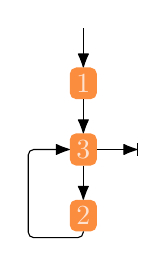
\begin{tikzpicture}[x=10mm,y=-7mm,inner sep=1pt]
          %% query parts
          \begin{scope}[every node/.style={codeEmph!25,draw=codeEmph,fill=codeEmph,rounded corners=2pt,inner sep=2pt,line width=0.8pt}]
            \node at (0,0.0) (start) {1};
            \node at (0,1.2) (check) {3};
            \node at (0,2.4) (step)  {2};
          \end{scope}
          \coordinate (through) at (-0.7,2.8);
          %% transitions (through check)
          \begin{scope}[goto/.tip={Latex[round,length=2mm]},return/.tip={Latex[round,length=2mm] Bar}]
            \draw[{goto}-]   (start) to +(0,-1.0);
            \draw[-{goto}]   (start) to (check);
            \draw[-{return}] (check) to +(0.7,0);
            \draw[-{goto}]   (check) to (step);
            %% back-to-check transitions
            \begin{scope}[rounded corners=2pt]
              \draw[-{goto}] (step) to (step |- through) to (through) to (through |- check) to (check);
            \end{scope}
          \end{scope}
        \end{tikzpicture}
      \end{figure}
    \end{column}
  \end{columns}
\end{frame}

\begin{frame}[fragile]
  \frametitle{``Trampolined Style''}

  \begin{columns}[c]
    \begin{column}{0.45\textwidth}
      \begin{figure}[t]
        \centering
        \scriptsize
        %% measure the width of xx in a listing
        \settowidth{\xx}{\lstinline[columns=fixed]{xx}}\setlength{\x}{0.5\xx}
        \setlength{\y}{2ex}
        \begin{tikzpicture}[x=\x,y=-\y,inner sep=0mm]
          \node[anchor=north west] at (0,0) {%
            \begin{lstlisting}[language=sql,gobble=14]
              WITH RECURSIVE
                cte(...) AS (
                  SELECT '%*\twemoji{rocket}*)' AS mode
                    UNION
                  SELECT
                    CASE mode
                      WHEN '%*\twemoji{rocket}*)'
                      THEN ...
                      WHEN '%*\twemoji{gear}*)'
                      THEN ...
                      WHEN '%*\twemoji{sewing needle}*)'
                      THEN ...
                      WHEN '%*\twemoji{person running: medium skin tone}*)'
                      THEN ...
                    END
                  FROM   cte
                  WHERE  mode != '%*\twemoji{chequered flag}*)'
                  )
                SELECT ...
                FROM   cte
                WHERE  ...;
            \end{lstlisting}%
          };
          \begin{pgfonlayer}{background}
            \begin{scope}[rounded corners=2pt]
              \fill[codebg] (-1.0,-0.5) rectangle (23.5,22.5);
              \fill[codeEmph,draw=codeEmph,line width=1.7pt] (2.5, 2.2) rectangle (22.5, 3.2);
              \fill[codeEmph!25]                             (4.0, 2.2) rectangle (22.5, 3.2);
              \fill[codeEmph,draw=codeEmph,line width=1.7pt] (2.5, 4.3) rectangle (22.5,15.8);
              \fill[codeEmph!25]                             (4.0, 4.3) rectangle (22.5,15.8);
              \fill[codeEmph,draw=codeEmph,line width=1.7pt] (2.5,16.9) rectangle (22.5,18.0);
              \fill[codeEmph!25]                             (4.0,16.9) rectangle (22.5,18.0);
            \end{scope}
            \begin{scope}[inner sep=1pt]
              \node[codeEmph!25] at (3.25, 2.7) {1};
              \node[codeEmph!25] at (3.25, 4.8) {2};
              \node[codeEmph!25] at (3.25,17.5) {3};
            \end{scope}
          \end{pgfonlayer}
        \end{tikzpicture}
      \end{figure}
    \end{column}
    \begin{column}{0.45\textwidth}
      \begin{figure}
        \centering
        \settowidth{\xx}{\twemoji{rocket}\twemoji{rocket}}\setlength{\x}{0.5\xx}
        \setlength{\y}{2ex}
        
\begin{tikzpicture}[x=\x,y=-\y,inner sep=1pt]
          %% query parts
          \begin{scope}[every node/.style={codeEmph,draw=codeEmph,fill=codeEmph!25,rounded corners=2pt,inner sep=2pt,line width=0.9pt}]
            \node at ( 0.0,0.0) (start)  {\twemoji{rocket}};
            \node at ( 0.0,2.0) (check)  {\twemoji{chequered flag}?};
            \node at (-2.4,4.0) (rocket) {\twemoji{rocket}};
            \node at (-0.8,4.0) (gear)   {\twemoji{gear}};
            \node at ( 0.8,4.0) (thread) {\twemoji{sewing needle}};
            \node at ( 2.4,4.0) (run)    {\twemoji{person running: medium skin tone}};
            \coordinate (check') at (2.56,2.0);
          \end{scope}
          \coordinate (through) at (-3.8,4.8);
          %% transitions (through check)
          \begin{scope}[goto/.tip={Latex[round,length=2mm]},return/.tip={Latex[round,length=2mm] Bar}]
            \draw[{goto}-]   (start)  to +(0,-1.5);
            \draw[-{goto}]   (start)  to (check);
            \draw[-{return}] (check') to +(1.5,0);
            \draw[-{goto}]   (check)  to [bend right=10] (rocket);
            \draw[-{goto}]   (check)  to [bend right=10] (gear);
            \draw[-{goto}]   (check)  to                 (thread);
            \draw[-{goto}]   (check)  to [bend left=10]  (run);
            %% back-to-check transitions
            \begin{scope}[rounded corners=2pt]
              \draw[-{goto}]       (run)    to (run    |- through) to (through) to (through |- check) to (check);
              \draw[shorten >=2pt] (thread) to (thread |- through) to (through);
              \draw[shorten >=2pt] (gear)   to (gear   |- through) to (through);
              \draw[shorten >=2pt] (rocket) to (rocket |- through) to (through);
            \end{scope}
          \end{scope}
          \begin{pgfonlayer}{background}
            \begin{scope}[rounded corners=2pt]
              \fill[codeEmph,draw=codeEmph,line width=0.9pt] (-0.5,-0.5) rectangle (2.0,0.5);
              \fill[codeEmph,draw=codeEmph,line width=0.9pt] (-1.0, 1.49) rectangle (2.5,2.5);
              \fill[codeEmph,draw=codeEmph,line width=0.9pt] (-2.9, 3.5) rectangle (4.4,4.5);
            \end{scope}
            \node[codeEmph!25] at (1.4,0) {1};
            \node[codeEmph!25] at (1.9,2) {3};
            \node[codeEmph!25] at (3.8,4) {2};
          \end{pgfonlayer}
        \end{tikzpicture}
      \end{figure}
    \end{column}
  \end{columns}
\end{frame}

\begin{frame}
  \frametitle{Befunge — Brainfuck but somehow weirder...}

  Sed iaculis \alert{dapibus gravida}. Morbi sed tortor erat, nec interdum arcu.
  Sed id lorem lectus. Quisque viverra augue id sem ornare non aliquam nibh
  tristique. Aenean in ligula nisl. Nulla sed tellus ipsum. Donec vestibulum
  ligula non lorem vulputate fermentum accumsan neque mollis.

  \bigskip % Vertical whitespace

  % Quote example
  \begin{quote}
    Sed diam enim, sagittis nec condimentum sit amet, ullamcorper sit amet libero. Aliquam vel dui orci, a porta odio.\\
    --- Someone, somewhere\ldots
  \end{quote}

  \bigskip % Vertical whitespace

  Nullam id suscipit ipsum. Aenean lobortis commodo sem, ut commodo leo gravida
  vitae. Pellentesque vehicula ante iaculis arcu pretium rutrum eget sit amet
  purus. Integer ornare nulla quis neque ultrices lobortis.
\end{frame}

\begin{frame}
  \frametitle{Lists}
  \framesubtitle{Bullet Points and Numbered Lists} % Optional subtitle

  \begin{itemize}
    \item Lorem ipsum dolor sit amet, consectetur adipiscing elit
    \item Aliquam blandit faucibus nisi, sit amet dapibus enim tempus
          \begin{itemize}
            \item Lorem ipsum dolor sit amet, consectetur adipiscing elit
            \item Nam cursus est eget velit posuere pellentesque
          \end{itemize}
    \item Nulla commodo, erat quis gravida posuere, elit lacus lobortis est, quis
          porttitor odio mauris at libero
  \end{itemize}

  \bigskip % Vertical whitespace

  \begin{enumerate}
    \item Nam cursus est eget velit posuere pellentesque
    \item Vestibulum faucibus velit a augue condimentum quis convallis nulla gravida
  \end{enumerate}
\end{frame}

\begin{frame}
  \frametitle{Blocks of Highlighted Text}

  \begin{block}{Block Title}
    Lorem ipsum dolor sit amet, consectetur adipiscing elit. Integer lectus nisl, ultricies in feugiat rutrum, porttitor sit amet augue.
  \end{block}

  \begin{exampleblock}{Example Block Title}
    Aliquam ut tortor mauris. Sed volutpat ante purus, quis accumsan.
  \end{exampleblock}

  \begin{alertblock}{Alert Block Title}
    Pellentesque sed tellus purus. Class aptent taciti sociosqu ad litora torquent per conubia nostra, per inceptos himenaeos.
  \end{alertblock}

  \begin{block}{} % Block without title
    Suspendisse tincidunt sagittis gravida. Curabitur condimentum, enim sed venenatis rutrum, ipsum neque consectetur orci.
  \end{block}
\end{frame}

\begin{frame}
  \frametitle{Multiple Columns}
  \framesubtitle{Subtitle} % Optional subtitle

  \begin{columns}[c] % The "c" option specifies centered vertical alignment while the "t" option is used for top vertical alignment
    \begin{column}{0.45\textwidth} % Left column width
      \textbf{Heading}
      \begin{enumerate}
        \item Statement
        \item Explanation
        \item Example
      \end{enumerate}
    \end{column}
    \begin{column}{0.5\textwidth} % Right column width
      Lorem ipsum dolor sit amet, consectetur adipiscing elit. Integer lectus nisl, ultricies in feugiat rutrum, porttitor sit amet augue. Aliquam ut tortor mauris. Sed volutpat ante purus, quis accumsan dolor.
    \end{column}
  \end{columns}
\end{frame}
